\section{Introduzione alle Reti Neurali}
\subsection{Il modello di McCulloch-Pitts}
Un modello pensato dai due tizi qui presenti,
\begin{itemize}
    \item Warren McCulloch
    \item Walter Pitts

\end{itemize}

Era formato da:
\begin{itemize}
    \item Un insieme di neuroni
    \item Un insieme di connessioni tra i neuroni
    \item Un insieme di pesi associati alle connessioni
    \item Una funzione di attivazione
    \item Una funzione di output
\end{itemize}

Quindi immaginiamo $x_1, x_2, \dots, x_n$ che vengono dati come input, e quello
che viene fuori è un valore di $y \in \{0,1\}$. Questo è un modello di
classificazione binaria.

In soldoni, in deep learning si usa un vettore di numeri per tirare fuori un
altro vettore di numeri.

Nella maggior parte del tempo, però, non lavoriamo solamente con i dati.
\begin{itemize}
    \item immagini
    \item Testo
    \item Audio
    \item \dots
\end{itemize}
Non ci sono concetti di foto, video, immagini. L'unico concetto che esiste
è quello dei numeri.

\subsection{Modello di Rosenblatt}
Qui il modello è leggermente diverso. Gli elementi in questo modello sono i
seguenti:
\begin{itemize}
    \item Valori di input: $x_i$
    \item Funzione di attivazione: $\phi$
    \item Pesi degli archi: $w_i$
    \item Bias: $b$
\end{itemize}

\begin{equation}
    h(x|w,b) = h(\sum_{i=1}^l w_i\cdot x_i -b) = h(\sum_{i=1}^l w_i\cdot x_i) = \textit{sign}(w^Tx)
\end{equation}

\textbf{Nota:} Quando il \textbf{bias} non viene specificato, allora
si assume che sia 0.

I pesi $w_i$ sono collegati archi che vanno da $x_i$ al prossimo neurone. Sia
il valore di input che il peso sono \textbf{numeri reali}. Non sono lo stesso
valore, hanno solamente il formato di \textit{reale} che è uguale tra loro. Ciò
che viene fatto è solamente la somma della prodotto tra ogni peso $w_i$ e $x_i$
\textbf{meno} il bias.

\textbf{La funzione di attivazione:} Dipende. Ogni funzione che ha \textit{2 stati} va bene per noi. Una funzione di attivazione può essere una qualsiasi che in un
punto ha valore 1 e in un altro ha valore -1.

\subsection{Esempio con 2 neuroni}.

Immaginiamo di avere un piano cartesiano con una retta che interseca in 2
punti.

\begin{equation}
    sign(w_1\cdot x_1 + w_2\cdot x_2)
\end{equation}

Il parametro della funzione non è altro che \textbf{l'equazione di una retta.}

In particolare, se consideriamo la reta che separa gli spazi del piano, vediamo
che la retta è \textbf{capace di separare 2 punti nel piano.}

\textbf{Cosa abbiamo}:
\begin{itemize}
    \item Un neurone
    \item 2 valori in input
    \item 2 pesi
\end{itemize}

Con la funzione di attivazione \textbf{sign} si avrà come output una retta che
separa dei punti.
\begin{tikzpicture}[scale=1.5]
    % Asse x
    \draw[->] (-2,0) -- (2,0) node[right] {$x$};
    % Asse y
    \draw[->] (0,-2) -- (0,2) node[above] {$y$};

    % Punto A
    \coordinate (A) at (-1.5,1);
    \fill[red] (A) circle (2pt) node[above left] {$A$};

    % Punto B
    \coordinate (B) at (1,0.5);
    \fill (B) circle (2pt) node[above right] {$B$};

    % Retta
    \draw[dashed] (-2,-0.25) -- (2,1.75) node[right] {$r$};
\end{tikzpicture}

\textbf{Nota}: Quando è utile avere un valore output che non è una separazione di punti in un piano? Nel caso della \textbf{regressione}.

\textbf{Oltre la funzione sign}:
\begin{itemize}
    \item Funzione di attivazione lineare
    \item Funzione di attivazione sigmoid
    \item Funzione di attivazione Tanh
\end{itemize}

\subsection{Rappresentazione le funzioni logiche}:

\subsubsection{AND}
Immaginiamo di avere:
\begin{itemize}
    \item $x_1,x_2 \in \{0,1\}$
    \item Bias= -30
    \item Funzione di attivazione: Logistica o Sigmoid
\end{itemize}

Come facciamo a rappresentare un AND?

\begin{equation}
    h(x)= g(-30+20x_1 +20x_2)
\end{equation}
\begin{center}
    \begin{tabular}{|c|c|c|}
        \hline
        $x_1$ & $x_2$ & $h(x)$ \\
        \hline
        0     & 0     & 1      \\
        0     & 1     & 0      \\
        1     & 0     & 0      \\
        1     & 1     & 1      \\
        \hline
    \end{tabular}
\end{center}

Lo stesso ragionamento vale per:
\begin{itemize}
    \item OR
    \item NOT
    \item (NOT $x_1$) AND (NOT $x_2$)
\end{itemize}

\subsubsection{Il problema dello XOR}
\begin{quote}
    Il percettrone non può imparare regioni che non sono linearmente separabili.
\end{quote}

\begin{figure}[H]
    \begin{center}
        \begin{tikzpicture}[scale=1.5][h!]
            % Asse x
            \draw[->] (-2,0) -- (2,0) node[right] {$x$};
            % Asse y
            \draw[->] (0,-2) -- (0,2) node[above] {$y$};

            % Punto A
            \coordinate (A) at (0,1);
            \fill[red] (A) circle (2pt) node[above left] {$A$};

            % Punto B
            \coordinate (B) at (0,0);
            \fill (B) circle (2pt) node[above right] {$B$};

            \coordinate (B) at (1,0);
            \fill (B)[red] circle (2pt) node[above right] {$B$};

            \coordinate (B) at (1,1);
            \fill (B) circle (2pt) node[above right] {$B$};
        \end{tikzpicture}
        \caption{XOR non possibile con 1 percettrone}
    \end{center}

\end{figure}

Come vediamo qui non possoamo tracciare una retta per dividere i due punti. In
questo caso ci serve una funzione \textbf{non lineare}.

La soluzione a questo problema è \textbf{aggiungere LAYER} alla rete neurale.
Aggiungere un layer significa aggiungere un neurone successivamente ad un
altro.

Maggiore è il numero di layer, maggiore diventa la potenza espressiva della
rete. Praticamente possiamo catturare qualsiasi cosa aggiungendo layer alla
rete. Questo è \textbf{il vero potere del deep learning}.

\usetikzlibrary{positioning}
\begin{figure}[H]
    \begin{center}

        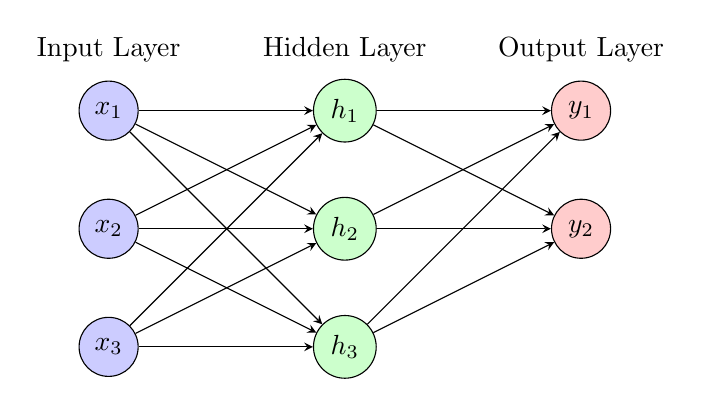
\begin{tikzpicture}[x=1.5cm, y=1.5cm, >=stealth]

            % Input Layer
            \foreach \i in {1,2,3}
            \node[circle, draw, fill=blue!20, minimum size=0.75cm] (I\i) at (0,-\i) {$x_{\i}$};

            % Hidden Layer
            \foreach \i in {1,2,3}
            \node[circle, draw, fill=green!20, minimum size=0.75cm] (H\i) at (2,-\i) {$h_{\i}$};

            % Output Layer
            \foreach \i in {1,2}
            \node[circle, draw, fill=red!20, minimum size=0.75cm] (O\i) at (4,-\i) {$y_{\i}$};

            % Connect Layers
            \foreach \i in {1,2,3}
            \foreach \j in {1,2,3}
            \draw[->] (I\i) -- (H\j);

            \foreach \i in {1,2,3}
            \foreach \j in {1,2}
            \draw[->] (H\i) -- (O\j);

            % Labels
            \node[above=0.5cm] at (I1) {Input Layer};
            \node[above=0.5cm] at (H1) {Hidden Layer};
            \node[above=0.5cm] at (O1) {Output Layer};

        \end{tikzpicture}
    \end{center}

\end{figure}